\documentclass[]{book}
\usepackage{lmodern}
\usepackage{amssymb,amsmath}
\usepackage{ifxetex,ifluatex}
\usepackage{fixltx2e} % provides \textsubscript
\ifnum 0\ifxetex 1\fi\ifluatex 1\fi=0 % if pdftex
  \usepackage[T1]{fontenc}
  \usepackage[utf8]{inputenc}
\else % if luatex or xelatex
  \ifxetex
    \usepackage{mathspec}
  \else
    \usepackage{fontspec}
  \fi
  \defaultfontfeatures{Ligatures=TeX,Scale=MatchLowercase}
\fi
% use upquote if available, for straight quotes in verbatim environments
\IfFileExists{upquote.sty}{\usepackage{upquote}}{}
% use microtype if available
\IfFileExists{microtype.sty}{%
\usepackage{microtype}
\UseMicrotypeSet[protrusion]{basicmath} % disable protrusion for tt fonts
}{}
\usepackage[margin=1in]{geometry}
\usepackage{hyperref}
\hypersetup{unicode=true,
            pdftitle={Aprender R: iniciación y perfeccionamiento},
            pdfauthor={François Rebaudo},
            pdfborder={0 0 0},
            breaklinks=true}
\urlstyle{same}  % don't use monospace font for urls
\usepackage{natbib}
\bibliographystyle{apalike}
\usepackage{color}
\usepackage{fancyvrb}
\newcommand{\VerbBar}{|}
\newcommand{\VERB}{\Verb[commandchars=\\\{\}]}
\DefineVerbatimEnvironment{Highlighting}{Verbatim}{commandchars=\\\{\}}
% Add ',fontsize=\small' for more characters per line
\usepackage{framed}
\definecolor{shadecolor}{RGB}{248,248,248}
\newenvironment{Shaded}{\begin{snugshade}}{\end{snugshade}}
\newcommand{\KeywordTok}[1]{\textcolor[rgb]{0.13,0.29,0.53}{\textbf{#1}}}
\newcommand{\DataTypeTok}[1]{\textcolor[rgb]{0.13,0.29,0.53}{#1}}
\newcommand{\DecValTok}[1]{\textcolor[rgb]{0.00,0.00,0.81}{#1}}
\newcommand{\BaseNTok}[1]{\textcolor[rgb]{0.00,0.00,0.81}{#1}}
\newcommand{\FloatTok}[1]{\textcolor[rgb]{0.00,0.00,0.81}{#1}}
\newcommand{\ConstantTok}[1]{\textcolor[rgb]{0.00,0.00,0.00}{#1}}
\newcommand{\CharTok}[1]{\textcolor[rgb]{0.31,0.60,0.02}{#1}}
\newcommand{\SpecialCharTok}[1]{\textcolor[rgb]{0.00,0.00,0.00}{#1}}
\newcommand{\StringTok}[1]{\textcolor[rgb]{0.31,0.60,0.02}{#1}}
\newcommand{\VerbatimStringTok}[1]{\textcolor[rgb]{0.31,0.60,0.02}{#1}}
\newcommand{\SpecialStringTok}[1]{\textcolor[rgb]{0.31,0.60,0.02}{#1}}
\newcommand{\ImportTok}[1]{#1}
\newcommand{\CommentTok}[1]{\textcolor[rgb]{0.56,0.35,0.01}{\textit{#1}}}
\newcommand{\DocumentationTok}[1]{\textcolor[rgb]{0.56,0.35,0.01}{\textbf{\textit{#1}}}}
\newcommand{\AnnotationTok}[1]{\textcolor[rgb]{0.56,0.35,0.01}{\textbf{\textit{#1}}}}
\newcommand{\CommentVarTok}[1]{\textcolor[rgb]{0.56,0.35,0.01}{\textbf{\textit{#1}}}}
\newcommand{\OtherTok}[1]{\textcolor[rgb]{0.56,0.35,0.01}{#1}}
\newcommand{\FunctionTok}[1]{\textcolor[rgb]{0.00,0.00,0.00}{#1}}
\newcommand{\VariableTok}[1]{\textcolor[rgb]{0.00,0.00,0.00}{#1}}
\newcommand{\ControlFlowTok}[1]{\textcolor[rgb]{0.13,0.29,0.53}{\textbf{#1}}}
\newcommand{\OperatorTok}[1]{\textcolor[rgb]{0.81,0.36,0.00}{\textbf{#1}}}
\newcommand{\BuiltInTok}[1]{#1}
\newcommand{\ExtensionTok}[1]{#1}
\newcommand{\PreprocessorTok}[1]{\textcolor[rgb]{0.56,0.35,0.01}{\textit{#1}}}
\newcommand{\AttributeTok}[1]{\textcolor[rgb]{0.77,0.63,0.00}{#1}}
\newcommand{\RegionMarkerTok}[1]{#1}
\newcommand{\InformationTok}[1]{\textcolor[rgb]{0.56,0.35,0.01}{\textbf{\textit{#1}}}}
\newcommand{\WarningTok}[1]{\textcolor[rgb]{0.56,0.35,0.01}{\textbf{\textit{#1}}}}
\newcommand{\AlertTok}[1]{\textcolor[rgb]{0.94,0.16,0.16}{#1}}
\newcommand{\ErrorTok}[1]{\textcolor[rgb]{0.64,0.00,0.00}{\textbf{#1}}}
\newcommand{\NormalTok}[1]{#1}
\usepackage{longtable,booktabs}
\usepackage{graphicx,grffile}
\makeatletter
\def\maxwidth{\ifdim\Gin@nat@width>\linewidth\linewidth\else\Gin@nat@width\fi}
\def\maxheight{\ifdim\Gin@nat@height>\textheight\textheight\else\Gin@nat@height\fi}
\makeatother
% Scale images if necessary, so that they will not overflow the page
% margins by default, and it is still possible to overwrite the defaults
% using explicit options in \includegraphics[width, height, ...]{}
\setkeys{Gin}{width=\maxwidth,height=\maxheight,keepaspectratio}
\IfFileExists{parskip.sty}{%
\usepackage{parskip}
}{% else
\setlength{\parindent}{0pt}
\setlength{\parskip}{6pt plus 2pt minus 1pt}
}
\setlength{\emergencystretch}{3em}  % prevent overfull lines
\providecommand{\tightlist}{%
  \setlength{\itemsep}{0pt}\setlength{\parskip}{0pt}}
\setcounter{secnumdepth}{5}
% Redefines (sub)paragraphs to behave more like sections
\ifx\paragraph\undefined\else
\let\oldparagraph\paragraph
\renewcommand{\paragraph}[1]{\oldparagraph{#1}\mbox{}}
\fi
\ifx\subparagraph\undefined\else
\let\oldsubparagraph\subparagraph
\renewcommand{\subparagraph}[1]{\oldsubparagraph{#1}\mbox{}}
\fi

%%% Use protect on footnotes to avoid problems with footnotes in titles
\let\rmarkdownfootnote\footnote%
\def\footnote{\protect\rmarkdownfootnote}

%%% Change title format to be more compact
\usepackage{titling}

% Create subtitle command for use in maketitle
\newcommand{\subtitle}[1]{
  \posttitle{
    \begin{center}\large#1\end{center}
    }
}

\setlength{\droptitle}{-2em}

  \title{Aprender R: iniciación y perfeccionamiento}
    \pretitle{\vspace{\droptitle}\centering\huge}
  \posttitle{\par}
    \author{François Rebaudo}
    \preauthor{\centering\large\emph}
  \postauthor{\par}
      \predate{\centering\large\emph}
  \postdate{\par}
    \date{2018-07-03}

\usepackage{booktabs}
\usepackage{longtable}
\usepackage[bf,singlelinecheck=off]{caption}

\setmainfont[UprightFeatures={SmallCapsFont=Arial}]{Arial} % AlegreyaSC-Regular % Alegreya

\usepackage{framed,color}
\definecolor{shadecolor}{RGB}{248,248,248}

\renewcommand{\textfraction}{0.05}
\renewcommand{\topfraction}{0.8}
\renewcommand{\bottomfraction}{0.8}
\renewcommand{\floatpagefraction}{0.75}

\renewenvironment{quote}{\begin{VF}}{\end{VF}}
\let\oldhref\href
\renewcommand{\href}[2]{#2\footnote{\url{#1}}}

\ifxetex
  \usepackage{letltxmacro}
  \setlength{\XeTeXLinkMargin}{1pt}
  \LetLtxMacro\SavedIncludeGraphics\includegraphics
  \def\includegraphics#1#{% #1 catches optional stuff (star/opt. arg.)
    \IncludeGraphicsAux{#1}%
  }%
  \newcommand*{\IncludeGraphicsAux}[2]{%
    \XeTeXLinkBox{%
      \SavedIncludeGraphics#1{#2}%
    }%
  }%
\fi

\makeatletter
\newenvironment{kframe}{%
\medskip{}
\setlength{\fboxsep}{.8em}
 \def\at@end@of@kframe{}%
 \ifinner\ifhmode%
  \def\at@end@of@kframe{\end{minipage}}%
  \begin{minipage}{\columnwidth}%
 \fi\fi%
 \def\FrameCommand##1{\hskip\@totalleftmargin \hskip-\fboxsep
 \colorbox{shadecolor}{##1}\hskip-\fboxsep
     % There is no \\@totalrightmargin, so:
     \hskip-\linewidth \hskip-\@totalleftmargin \hskip\columnwidth}%
 \MakeFramed {\advance\hsize-\width
   \@totalleftmargin\z@ \linewidth\hsize
   \@setminipage}}%
 {\par\unskip\endMakeFramed%
 \at@end@of@kframe}
\makeatother

\makeatletter
\@ifundefined{Shaded}{
}{\renewenvironment{Shaded}{\begin{kframe}}{\end{kframe}}}
\makeatother

\newenvironment{rmdblock}[1]
  {
  \begin{itemize}
  \renewcommand{\labelitemi}{
    \raisebox{-.7\height}[0pt][0pt]{
      {\setkeys{Gin}{width=3em,keepaspectratio}\includegraphics{myIcons/#1}} %FR
    }
  }
  \setlength{\fboxsep}{1em}
  \begin{kframe}
  \item
  }
  {
  \end{kframe}
  \end{itemize}
  }
\newenvironment{rmdnote}      %FR
  {\begin{rmdblock}{note}}    %FR
  {\end{rmdblock}}            %FR
\newenvironment{rmdstyle}     %FR
  {\begin{rmdblock}{style}}   %FR
  {\end{rmdblock}}            %FR
\newenvironment{rmdcaution}
  {\begin{rmdblock}{caution}}
  {\end{rmdblock}}
\newenvironment{rmdimportant}
  {\begin{rmdblock}{important}}
  {\end{rmdblock}}
\newenvironment{rmdtip}
  {\begin{rmdblock}{tip}}
  {\end{rmdblock}}
\newenvironment{rmdwarning}
  {\begin{rmdblock}{warning}}
  {\end{rmdblock}}

\usepackage{makeidx}
\makeindex

\urlstyle{tt}

\usepackage{amsthm}
\makeatletter
\def\thm@space@setup{%
  \thm@preskip=8pt plus 2pt minus 4pt
  \thm@postskip=\thm@preskip
}
\makeatother

\mainmatter

\begin{document}
\maketitle

{
\setcounter{tocdepth}{1}
\tableofcontents
}
\chapter{Agradecimientos}\label{remerciements}

Agradezco a todos los colaboradores que ayudaron a mejorar este libro
con sus consejos, sugerencias de cambios y correcciones:

=\textgreater{} lista para actualizar en la publicación.

Las versiones de gitbook, html y epub de este libro usan los iconos de
fuente abierta de Font Awesome (\url{https://fontawesome.com}). La
versión en PDF utiliza los iconos del proyecto Tango disponibles en
openclipart (\url{https://openclipart.org/}). Este libro fue escrito con
el paquete R bookdown (\url{https://bookdown.org/}). El código fuente
está disponible en GitHub (\url{https://github.com/frareb/myRBook_SP}).
La compilación usa Travis CI (\url{https://travis-ci.org}). La versión
en línea se aloja y actualiza a través de Netlify
(\url{http://myrbooksp.netlify.com/}).

\chapter{Licencia}\label{licence}

Licencia Reconocimiento-NoComercial-SinObraDerivada 3.0 España (CC
BY-NC-ND 3.0 ES ;
\url{https://creativecommons.org/licenses/by-nc-nd/3.0/es/})

Esto es un resumen inteligible para humanos (y no un sustituto) de la
licencia.

\textbf{Usted es libre de:}

\begin{itemize}
\tightlist
\item
  Compartir --- copiar y redistribuir el material en cualquier medio o
  formato.
\item
  El licenciador no puede revocar estas libertades mientras cumpla con
  los términos de la licencia.
\end{itemize}

\textbf{Bajo las condiciones siguientes:}

\begin{itemize}
\item
  Reconocimiento --- Debe reconocer adecuadamente la autoría,
  proporcionar un enlace a la licencia e indicar si se han realizado
  cambios\textless{}. Puede hacerlo de cualquier manera razonable, pero
  no de una manera que sugiera que tiene el apoyo del licenciador o lo
  recibe por el uso que hace.
\item
  NoComercial --- No puede utilizar el material para una finalidad
  comercial.
\item
  SinObraDerivada --- Si remezcla, transforma o crea a partir del
  material, no puede difundir el material modificado.
\item
  No hay restricciones adicionales --- No puede aplicar términos legales
  o medidas tecnológicas que legalmente restrinjan realizar aquello que
  la licencia permite.
\end{itemize}

\textbf{Avisos: }

No tiene que cumplir con la licencia para aquellos elementos del
material en el dominio público o cuando su utilización esté permitida
por la aplicación de una excepción o un límite. No se dan garantías. La
licencia puede no ofrecer todos los permisos necesarios para la
utilización prevista. Por ejemplo, otros derechos como los de
publicidad, privacidad, o los derechos morales pueden limitar el uso del
material.

\chapter{introducción}\label{intro}

\section{Por qué apprender R}\label{por-que-apprender-r}

\section{Este libro}\label{este-libro}

\section{Lectura adicional en
español}\label{lectura-adicional-en-espanol}

\begin{itemize}
\tightlist
\item
  R para Principiantes, Emmanuel Paradis
  (\url{https://cran.r-project.org/doc/contrib/rdebuts_es.pdf})
\item
  xxx
\end{itemize}

\part{Conceptos básicos}\label{part-conceptos-basicos}

\chapter{Primeros pasos}\label{premiersPas}

\section{Instalar R}\label{instalar-r}

El programa para instalar el software R se puede descargar desde el
sitio web de R: \url{https://www.r-project.org/}. En el sitio web de R,
primero es necesario elegir un espejo CRAN (servidor desde el que
descargar R, el más cercano a su ubicación geográfica), luego descargue
el archivo \emph{base}. Los usuarios de Linux pueden preferir un
\texttt{sudo\ apt-get\ install\ r-base}.

\begin{rmdnote}
El software R se puede descargar de muchos servidores CRAN
(Comprehensive R Archive Network) de todo el mundo. Estos servidores se
llaman espejos. La elección del espejo es manual. Información adicional
como esta nota siempre estará representada con este pictograma
\emph{información}.
\end{rmdnote}

\section{R como calculadora}\label{r-como-calculadora}

Una vez que se inicia el programa, aparece una ventana cuya apariencia
puede variar dependiendo de su sistema operativo (Figura
\ref{fig:screenCapConsole}). Esta ventana se llama \emph{consola}.

\begin{figure}
\centering
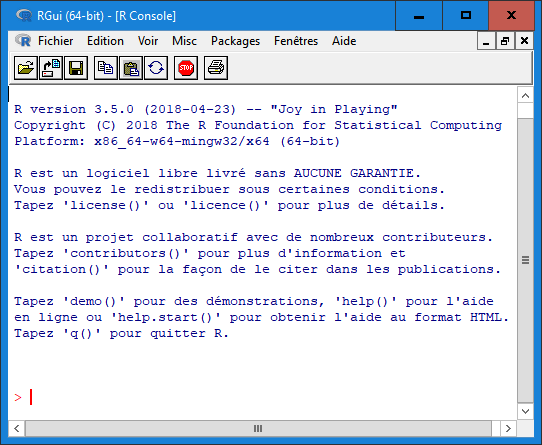
\includegraphics{myFigures/screencap_rConsoleFR.png}
\caption{\label{fig:screenCapConsole}Captura de pantalla de la consola R en
Windows.\label{fig:screenCapConsole}}
\end{figure}

La consola corresponde a la interfaz donde se interpretará el código, es
decir, donde el código será transformado en lenguaje de máquina,
ejecutado por la computadora y retransmitido en forma legible por
humanos. Esto corresponde a la pantalla de una calculadora (Figura
\ref{fig:screenCapConsoleCal}). Así es como se usará R más adelante en
esta sección.

\begin{rmdnote}
A lo largo de este libro, los ejemplos del código R aparecerán sobre un
fondo gris. Se pueden copiar y pegar directamente en la consola, aunque
es mejor reproducir escribiendo los ejemplos en la consola (o más
adelante en los scripts). El resultado de lo que se envía en la consola
también aparecerá en un fondo gris con \texttt{\#\#} delante del código
para hacer la distinción entre el código y el resultado del código.
\end{rmdnote}

\begin{figure}
\centering
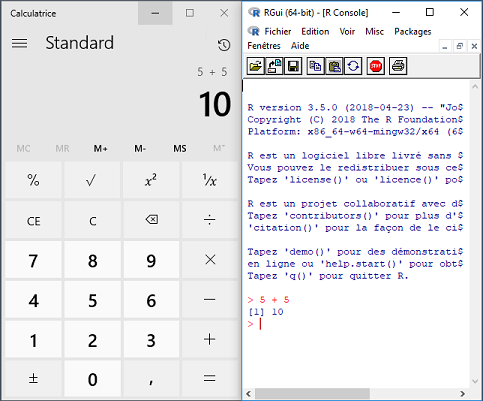
\includegraphics{myFigures/screencap_rConsoleCalculatrice.png}
\caption{\label{fig:screenCapConsoleCal}Captura de pantalla de la consola R
al lado de la calculadora de Windows.\label{fig:screenCapConsoleCal}}
\end{figure}

\subsection{Los operadores
aritméticos}\label{los-operadores-aritmeticos}

\begin{Shaded}
\begin{Highlighting}[]
\DecValTok{5} \OperatorTok{+}\StringTok{ }\DecValTok{5}
\end{Highlighting}
\end{Shaded}

\begin{verbatim}
## [1] 10
\end{verbatim}

Si escribimos \texttt{5\ +\ 5} en la consola y luego \texttt{Enter}, el
resultado aparece precedido por el número {[}1{]} entre corchetes. Este
número corresponde al número del resultado (en nuestro caso, solo hay un
resultado, volveremos a este aspecto más adelante). También podemos
observar en este ejemplo el uso de espacios antes y después del signo
\texttt{+}. Estos espacios no son necesarios, pero permiten que el
código sea más legible para los humanos (es decir, más agradable de leer
tanto para nosotros como para las personas con las que queremos
compartir nuestro código). Los operadores aritméticos disponibles en R
se resumen en la tabla \ref{tab:tabOpAri}.

\begin{table}

\caption{\label{tab:tabOpAri}Operadores aritméticos.\label{tab:tabOpAri}}
\centering
\begin{tabular}[t]{l|l}
\hline
Label & Operador\\
\hline
adición & +\\
\hline
resta & -\\
\hline
multiplicación & *\\
\hline
división & /\\
\hline
potencia & \textasciicircum{}\\
\hline
módulo & \%\%\\
\hline
cociente decimal & \%/\%\\
\hline
\end{tabular}
\end{table}

Clásicamente, las multiplicaciones y divisiones tienen prioridad sobre
las adiciones y sustracciones. Si es necesario, podemos usar paréntesis.

\begin{Shaded}
\begin{Highlighting}[]
\DecValTok{5} \OperatorTok{+}\StringTok{ }\DecValTok{5} \OperatorTok{*}\StringTok{ }\DecValTok{2}
\end{Highlighting}
\end{Shaded}

\begin{verbatim}
## [1] 15
\end{verbatim}

\begin{Shaded}
\begin{Highlighting}[]
\NormalTok{(}\DecValTok{5} \OperatorTok{+}\StringTok{ }\DecValTok{5}\NormalTok{) }\OperatorTok{*}\StringTok{ }\DecValTok{2}
\end{Highlighting}
\end{Shaded}

\begin{verbatim}
## [1] 20
\end{verbatim}

\begin{Shaded}
\begin{Highlighting}[]
\NormalTok{(}\DecValTok{5} \OperatorTok{+}\StringTok{ }\DecValTok{5}\NormalTok{) }\OperatorTok{*}\StringTok{ }\NormalTok{(}\DecValTok{2} \OperatorTok{+}\StringTok{ }\DecValTok{2}\NormalTok{)}
\end{Highlighting}
\end{Shaded}

\begin{verbatim}
## [1] 40
\end{verbatim}

\begin{Shaded}
\begin{Highlighting}[]
\NormalTok{(}\DecValTok{5} \OperatorTok{+}\StringTok{ }\DecValTok{5}\NormalTok{) }\OperatorTok{*}\StringTok{ }\NormalTok{((}\DecValTok{2} \OperatorTok{+}\StringTok{ }\DecValTok{2}\NormalTok{) }\OperatorTok{/}\StringTok{ }\DecValTok{3}\NormalTok{)}\OperatorTok{^}\DecValTok{2}
\end{Highlighting}
\end{Shaded}

\begin{verbatim}
## [1] 17.77778
\end{verbatim}

El operador de módulo corresponde al resto de la división euclidiana. Se
usa en ciencias de la computación, por ejemplo, para saber si un número
es par o impar (un número módulo 2 devolverá 1 si es impar y 0 si es
par).

\begin{Shaded}
\begin{Highlighting}[]
\DecValTok{451} \OperatorTok\StringTok{ }\DecValTok{2}
\end{Highlighting}
\end{Shaded}

\begin{verbatim}
## [1] 1
\end{verbatim}

\begin{Shaded}
\begin{Highlighting}[]
\DecValTok{288} \OperatorTok\StringTok{ }\DecValTok{2}
\end{Highlighting}
\end{Shaded}

\begin{verbatim}
## [1] 0
\end{verbatim}

\begin{Shaded}
\begin{Highlighting}[]
\NormalTok{(}\DecValTok{5} \OperatorTok{+}\StringTok{ }\DecValTok{5} \OperatorTok{*}\StringTok{ }\DecValTok{2}\NormalTok{) }\OperatorTok\StringTok{ }\DecValTok{2}
\end{Highlighting}
\end{Shaded}

\begin{verbatim}
## [1] 1
\end{verbatim}

\begin{Shaded}
\begin{Highlighting}[]
\NormalTok{((}\DecValTok{5} \OperatorTok{+}\StringTok{ }\DecValTok{5}\NormalTok{) }\OperatorTok{*}\StringTok{ }\DecValTok{2}\NormalTok{) }\OperatorTok\StringTok{ }\DecValTok{2}
\end{Highlighting}
\end{Shaded}

\begin{verbatim}
## [1] 0
\end{verbatim}

R también incorpora algunas constantes que incluyen \texttt{pi}. Además,
el signo infinito está representado por \texttt{Inf}.

\begin{Shaded}
\begin{Highlighting}[]
\NormalTok{pi}
\end{Highlighting}
\end{Shaded}

\begin{verbatim}
## [1] 3.141593
\end{verbatim}

\begin{Shaded}
\begin{Highlighting}[]
\NormalTok{pi }\OperatorTok{*}\StringTok{ }\DecValTok{5}\OperatorTok{^}\DecValTok{2}
\end{Highlighting}
\end{Shaded}

\begin{verbatim}
## [1] 78.53982
\end{verbatim}

\begin{Shaded}
\begin{Highlighting}[]
\DecValTok{1}\OperatorTok{/}\DecValTok{0}
\end{Highlighting}
\end{Shaded}

\begin{verbatim}
## [1] Inf
\end{verbatim}

\begin{rmdstyle}
el \emph{estilo} del código es importante porque el código está
destinado a ser leído por nosotros y por otras personas. Para tener un
estilo legible, se recomienda colocar espacios antes y después de los
operadores aritméticos, excepto ``*'', ``/'' y ``\^{}'', aunque a veces
es útil agregarlos como es el caso en nuestro ejemplos. La información
sobre el \emph{estilo} siempre estará representada con este pictograma
para que sea fácilmente identificable.
\end{rmdstyle}

\subsection{Los operadores
comparativos}\label{los-operadores-comparativos}

Sin embargo, R es mucho más que una simple calculadora porque permite
otro tipo de operadores: operadores de comparación. Sirven como su
nombre sugiere \emph{comparar} los valores (Table \ref{tab:tabOpCom}).

\begin{table}

\caption{\label{tab:tabOpCom}Operadores de comparación.\label{tab:tabOpCom}}
\centering
\begin{tabular}[t]{l|l}
\hline
Label & Operador\\
\hline
más pequeño que & <\\
\hline
mayor que & >\\
\hline
más pequeño o igual a & <=\\
\hline
más grande o igual a & >=\\
\hline
igual a & ==\\
\hline
diferente de & !=\\
\hline
\end{tabular}
\end{table}

Por ejemplo, si queremos saber si un numero es más grande que otro,
podemos escribir:

\begin{Shaded}
\begin{Highlighting}[]
\DecValTok{5} \OperatorTok{>}\StringTok{ }\DecValTok{3} 
\end{Highlighting}
\end{Shaded}

\begin{verbatim}
## [1] TRUE
\end{verbatim}

R devuelve \texttt{TRUE} si la comparación es verdadera y \texttt{FALSE}
si la comparación es falsa.

\begin{Shaded}
\begin{Highlighting}[]
\DecValTok{5} \OperatorTok{>}\StringTok{ }\DecValTok{3}
\end{Highlighting}
\end{Shaded}

\begin{verbatim}
## [1] TRUE
\end{verbatim}

\begin{Shaded}
\begin{Highlighting}[]
\DecValTok{2} \OperatorTok{<}\StringTok{ }\FloatTok{1.5}
\end{Highlighting}
\end{Shaded}

\begin{verbatim}
## [1] FALSE
\end{verbatim}

\begin{Shaded}
\begin{Highlighting}[]
\DecValTok{2} \OperatorTok{<=}\StringTok{ }\DecValTok{2}
\end{Highlighting}
\end{Shaded}

\begin{verbatim}
## [1] TRUE
\end{verbatim}

\begin{Shaded}
\begin{Highlighting}[]
\FloatTok{3.2} \OperatorTok{>=}\StringTok{ }\FloatTok{1.5}
\end{Highlighting}
\end{Shaded}

\begin{verbatim}
## [1] TRUE
\end{verbatim}

Podemos combinar operadores aritméticos con operadores de comparación.

\begin{Shaded}
\begin{Highlighting}[]
\NormalTok{(}\DecValTok{5} \OperatorTok{+}\StringTok{ }\DecValTok{8}\NormalTok{) }\OperatorTok{>}\StringTok{ }\NormalTok{(}\DecValTok{3} \OperatorTok{*}\StringTok{ }\DecValTok{45}\OperatorTok{/}\DecValTok{2}\NormalTok{) }
\end{Highlighting}
\end{Shaded}

\begin{verbatim}
## [1] FALSE
\end{verbatim}

\begin{rmdstyle}
En la comparación \texttt{(5\ +\ 8)\ \textgreater{}\ (3\ *\ 45/2)} no se
necesitan paréntesis, pero permiten que el código sea más fácil de leer.
\end{rmdstyle}

Un operador de comparación particular es \emph{igual a}. Veremos en la
siguiente sección que el signo \texttt{=} está reservado para otro uso:
permite asignar un valor a un objeto. El operador de comparación
\emph{igual a} debe ser diferente, por eso R usa \texttt{==}.

\begin{Shaded}
\begin{Highlighting}[]
\DecValTok{42} \OperatorTok{==}\StringTok{ }\DecValTok{53}
\end{Highlighting}
\end{Shaded}

\begin{verbatim}
## [1] FALSE
\end{verbatim}

\begin{Shaded}
\begin{Highlighting}[]
\DecValTok{58} \OperatorTok{==}\StringTok{ }\DecValTok{58}
\end{Highlighting}
\end{Shaded}

\begin{verbatim}
## [1] TRUE
\end{verbatim}

Otro operador particular es \emph{diferente de}. Se usa con \emph{un
signo de interrogación} seguido de \emph{igual}, \texttt{!\ =}. Este
operador permite obtener la respuesta opuesta a \texttt{==}.

\begin{Shaded}
\begin{Highlighting}[]
\DecValTok{42} \OperatorTok{==}\StringTok{ }\DecValTok{53}
\end{Highlighting}
\end{Shaded}

\begin{verbatim}
## [1] FALSE
\end{verbatim}

\begin{Shaded}
\begin{Highlighting}[]
\DecValTok{42} \OperatorTok{!=}\StringTok{ }\DecValTok{53}
\end{Highlighting}
\end{Shaded}

\begin{verbatim}
## [1] TRUE
\end{verbatim}

\begin{Shaded}
\begin{Highlighting}[]
\NormalTok{(}\DecValTok{3} \OperatorTok{+}\StringTok{ }\DecValTok{2}\NormalTok{) }\OperatorTok{!=}\StringTok{ }\DecValTok{5}
\end{Highlighting}
\end{Shaded}

\begin{verbatim}
## [1] FALSE
\end{verbatim}

\begin{Shaded}
\begin{Highlighting}[]
\DecValTok{10}\OperatorTok{/}\DecValTok{2} \OperatorTok{==}\StringTok{ }\DecValTok{5}
\end{Highlighting}
\end{Shaded}

\begin{verbatim}
## [1] TRUE
\end{verbatim}

R usa \texttt{TRUE} y \texttt{FALSE}, que también son valores que se
pueden probar con operadores de comparación. Pero R también asigna un
valor a \texttt{TRUE} y \texttt{FALSE}:

\begin{Shaded}
\begin{Highlighting}[]
\OtherTok{TRUE} \OperatorTok{==}\StringTok{ }\OtherTok{TRUE}
\end{Highlighting}
\end{Shaded}

\begin{verbatim}
## [1] TRUE
\end{verbatim}

\begin{Shaded}
\begin{Highlighting}[]
\OtherTok{TRUE} \OperatorTok{>}\StringTok{ }\OtherTok{FALSE}
\end{Highlighting}
\end{Shaded}

\begin{verbatim}
## [1] TRUE
\end{verbatim}

\begin{Shaded}
\begin{Highlighting}[]
\DecValTok{1} \OperatorTok{==}\StringTok{ }\OtherTok{TRUE}
\end{Highlighting}
\end{Shaded}

\begin{verbatim}
## [1] TRUE
\end{verbatim}

\begin{Shaded}
\begin{Highlighting}[]
\DecValTok{0} \OperatorTok{==}\StringTok{ }\OtherTok{FALSE}
\end{Highlighting}
\end{Shaded}

\begin{verbatim}
## [1] TRUE
\end{verbatim}

\begin{Shaded}
\begin{Highlighting}[]
\OtherTok{TRUE} \OperatorTok{+}\StringTok{ }\DecValTok{1}
\end{Highlighting}
\end{Shaded}

\begin{verbatim}
## [1] 2
\end{verbatim}

\begin{Shaded}
\begin{Highlighting}[]
\OtherTok{FALSE} \OperatorTok{+}\StringTok{ }\DecValTok{1}
\end{Highlighting}
\end{Shaded}

\begin{verbatim}
## [1] 1
\end{verbatim}

\begin{Shaded}
\begin{Highlighting}[]
\NormalTok{(}\OtherTok{FALSE} \OperatorTok{+}\StringTok{ }\DecValTok{1}\NormalTok{) }\OperatorTok{==}\StringTok{ }\OtherTok{TRUE}
\end{Highlighting}
\end{Shaded}

\begin{verbatim}
## [1] TRUE
\end{verbatim}

El valor de \texttt{TRUE} es 1 y el valor de \texttt{FALSE} es 0.
Veremos más adelante cómo usar esta información en los próximos
capítulos.

R es también un lenguaje relativamente permisivo, significa que admite
cierta flexibilidad en la forma de escribir el código. Debatir sobre la
idoneidad de esta flexibilidad está fuera del alcance de este libro,
pero podemos encontrar en el código R en Internet o en otras obras el
atajo \texttt{T} para \texttt{TRUE} y \texttt{F} for \texttt{FALSE}.

\begin{Shaded}
\begin{Highlighting}[]
\NormalTok{T }\OperatorTok{==}\StringTok{ }\OtherTok{TRUE}
\end{Highlighting}
\end{Shaded}

\begin{verbatim}
## [1] TRUE
\end{verbatim}

\begin{Shaded}
\begin{Highlighting}[]
\NormalTok{F }\OperatorTok{==}\StringTok{ }\OtherTok{FALSE}
\end{Highlighting}
\end{Shaded}

\begin{verbatim}
## [1] TRUE
\end{verbatim}

\begin{Shaded}
\begin{Highlighting}[]
\NormalTok{T }\OperatorTok{==}\StringTok{ }\DecValTok{1}
\end{Highlighting}
\end{Shaded}

\begin{verbatim}
## [1] TRUE
\end{verbatim}

\begin{Shaded}
\begin{Highlighting}[]
\NormalTok{F }\OperatorTok{==}\StringTok{ }\DecValTok{0}
\end{Highlighting}
\end{Shaded}

\begin{verbatim}
## [1] TRUE
\end{verbatim}

\begin{Shaded}
\begin{Highlighting}[]
\NormalTok{(F }\OperatorTok{+}\StringTok{ }\DecValTok{1}\NormalTok{) }\OperatorTok{==}\StringTok{ }\OtherTok{TRUE}
\end{Highlighting}
\end{Shaded}

\begin{verbatim}
## [1] TRUE
\end{verbatim}

Aunque esta forma de referirse a \texttt{TRUE} y \texttt{FALSE} por
\texttt{T} y \texttt{F} está bastante extendida, en este libro siempre
usaremos \texttt{TRUE} y \texttt{FALSE} para que el código sea más fácil
de leer. Como mencionado anterioramente, el objetivo de un código no
solo es ser funcional sino también fácil de leer y volver a leer.

\subsection{Los operadores lógicos}\label{los-operadores-logicos}

Hay un último tipo de operador, los operadores lógicos. Son útiles para
combinar operadores de comparación (Table \ref{tab:tabOpLog}).

\begin{table}

\caption{\label{tab:tabOpLog}Operadores lógicos.\label{tab:tabOpLog}}
\centering
\begin{tabular}[t]{l|l}
\hline
Label & Operador\\
\hline
no es & !\\
\hline
y & \&\\
\hline
o & |\\
\hline
o exclusivo & xor()\\
\hline
\end{tabular}
\end{table}

\begin{Shaded}
\begin{Highlighting}[]
\OperatorTok{!}\OtherTok{TRUE}
\end{Highlighting}
\end{Shaded}

\begin{verbatim}
## [1] FALSE
\end{verbatim}

\begin{Shaded}
\begin{Highlighting}[]
\OperatorTok{!}\OtherTok{FALSE}
\end{Highlighting}
\end{Shaded}

\begin{verbatim}
## [1] TRUE
\end{verbatim}

\begin{Shaded}
\begin{Highlighting}[]
\NormalTok{((}\DecValTok{3} \OperatorTok{+}\StringTok{ }\DecValTok{2}\NormalTok{) }\OperatorTok{==}\StringTok{ }\DecValTok{5}\NormalTok{) }\OperatorTok{&}\StringTok{ }\NormalTok{((}\DecValTok{3} \OperatorTok{+}\StringTok{ }\DecValTok{3}\NormalTok{) }\OperatorTok{==}\StringTok{ }\DecValTok{5}\NormalTok{)}
\end{Highlighting}
\end{Shaded}

\begin{verbatim}
## [1] FALSE
\end{verbatim}

\begin{Shaded}
\begin{Highlighting}[]
\NormalTok{((}\DecValTok{3} \OperatorTok{+}\StringTok{ }\DecValTok{2}\NormalTok{) }\OperatorTok{==}\StringTok{ }\DecValTok{5}\NormalTok{) }\OperatorTok{&}\StringTok{ }\NormalTok{((}\DecValTok{3} \OperatorTok{+}\StringTok{ }\DecValTok{3}\NormalTok{) }\OperatorTok{==}\StringTok{ }\DecValTok{6}\NormalTok{)}
\end{Highlighting}
\end{Shaded}

\begin{verbatim}
## [1] TRUE
\end{verbatim}

\begin{Shaded}
\begin{Highlighting}[]
\NormalTok{(}\DecValTok{3} \OperatorTok{<}\StringTok{ }\DecValTok{5}\NormalTok{) }\OperatorTok{&}\StringTok{ }\NormalTok{(}\DecValTok{5} \OperatorTok{<}\StringTok{ }\DecValTok{5}\NormalTok{)}
\end{Highlighting}
\end{Shaded}

\begin{verbatim}
## [1] FALSE
\end{verbatim}

\begin{Shaded}
\begin{Highlighting}[]
\NormalTok{(}\DecValTok{3} \OperatorTok{<}\StringTok{ }\DecValTok{5}\NormalTok{) }\OperatorTok{&}\StringTok{ }\NormalTok{(}\DecValTok{5} \OperatorTok{<=}\StringTok{ }\DecValTok{5}\NormalTok{)}
\end{Highlighting}
\end{Shaded}

\begin{verbatim}
## [1] TRUE
\end{verbatim}

El operador lógico \texttt{xor()} es \emph{o exclusivo}. Es decir, uno
de los dos \textbf{argumentos} de la \textbf{función} \texttt{xor()}
debe ser verdadero, pero no ambos. Más adelante volveremos a las
\textbf{funciones} y sus \textbf{argumentos}, pero recuerde que
identificamos una función por sus paréntesis que contienen argumentos
separados por comas.

\begin{Shaded}
\begin{Highlighting}[]
\KeywordTok{xor}\NormalTok{((}\DecValTok{3} \OperatorTok{+}\StringTok{ }\DecValTok{2}\NormalTok{) }\OperatorTok{==}\StringTok{ }\DecValTok{5}\NormalTok{, (}\DecValTok{3} \OperatorTok{+}\StringTok{ }\DecValTok{3}\NormalTok{) }\OperatorTok{==}\StringTok{ }\DecValTok{6}\NormalTok{)}
\end{Highlighting}
\end{Shaded}

\begin{verbatim}
## [1] FALSE
\end{verbatim}

\begin{Shaded}
\begin{Highlighting}[]
\KeywordTok{xor}\NormalTok{((}\DecValTok{3} \OperatorTok{+}\StringTok{ }\DecValTok{2}\NormalTok{) }\OperatorTok{==}\StringTok{ }\DecValTok{5}\NormalTok{, (}\DecValTok{3} \OperatorTok{+}\StringTok{ }\DecValTok{2}\NormalTok{) }\OperatorTok{==}\StringTok{ }\DecValTok{6}\NormalTok{)}
\end{Highlighting}
\end{Shaded}

\begin{verbatim}
## [1] TRUE
\end{verbatim}

\begin{Shaded}
\begin{Highlighting}[]
\KeywordTok{xor}\NormalTok{((}\DecValTok{3} \OperatorTok{+}\StringTok{ }\DecValTok{3}\NormalTok{) }\OperatorTok{==}\StringTok{ }\DecValTok{5}\NormalTok{, (}\DecValTok{3} \OperatorTok{+}\StringTok{ }\DecValTok{2}\NormalTok{) }\OperatorTok{==}\StringTok{ }\DecValTok{6}\NormalTok{)}
\end{Highlighting}
\end{Shaded}

\begin{verbatim}
## [1] FALSE
\end{verbatim}

\begin{Shaded}
\begin{Highlighting}[]
\KeywordTok{xor}\NormalTok{((}\DecValTok{3} \OperatorTok{+}\StringTok{ }\DecValTok{3}\NormalTok{) }\OperatorTok{==}\StringTok{ }\DecValTok{5}\NormalTok{, (}\DecValTok{3} \OperatorTok{+}\StringTok{ }\DecValTok{3}\NormalTok{) }\OperatorTok{==}\StringTok{ }\DecValTok{6}\NormalTok{)}
\end{Highlighting}
\end{Shaded}

\begin{verbatim}
## [1] TRUE
\end{verbatim}

\begin{rmdstyle}
Se recomienda que las comas \texttt{,} sean seguidas de un espacio para
que el código sea más agradable de leer.
\end{rmdstyle}

\subsection{Ayuda a los operadores}\label{ayuda-a-los-operadores}

El archivo de ayuda en inglés sobre operadores aritméticos se puede
obtener con el comando \texttt{?\textquotesingle{}+\textquotesingle{}}.
El de los operadores de comparación con el comando
\texttt{?\textquotesingle{}==\textquotesingle{}} y el de los operadores
lógicos con el comando \texttt{?\textquotesingle{}\&\textquotesingle{}}.

\section{El concepto de objeto}\label{el-concepto-de-objeto}

Un aspecto importante de la programación con R, pero también la
programación en general es la noción de objeto. Como se indica en la
página web de wikipedia
(\url{https://ia.wikipedia.org/wiki/Objecto_(informatica)}), en ciencias
de la computación, un objeto es un \emph{contenedor}, es decir, algo que
contendrá información. La inforamción contenida en un objeto puede ser
muy diversa, pero por el momento contendremos en un objeto el número 5.
Para hacer esto (y para reutilizarlo más adelante), debemos darle un
nombre a nuestro objeto. Con R, los nombres de los objetos no deben
contener caracteres especiales como \emph{\^{} \$ ? \textbar{} + ()
{[}{]} \{\}}, entre otros. No deben comenzar con un número ni contener
espacios. El nombre del objeto debe ser representativo de lo que
contiene, sin ser demasiado corto ni demasiado largo. Imagine que
nuestro número 5 corresponde al número de repeticiones de un
experimento. Nos gustaría darle un nombre que se refiera a \emph{numero}
y \emph{repeticiones}, que podríamos reducir a \emph{nbr} y \emph{rep},
respectivamente (\emph{nbr} para number en ingles). Hay varias
posibilidades que son bastante comunes bajo R:

\begin{itemize}
\tightlist
\item
  la separación mediante \emph{guión bajo} (underscore):
  \texttt{nbr\_rep}
\item
  la separación mediante el carácter \emph{punto}: \texttt{nbr.rep}
\item
  el uso de letras minúsculas: \texttt{nbrrep}
\item
  el estilo \emph{lowerCamelCase} que consiste en una primera palabra en
  minúscula y la primera letra de las siguientes palabras con una letra
  mayúscula: \texttt{nbrRep}
\item
  el estilo \emph{UpperCamelCase} donde cada palabra comienza con una
  letra mayúscula: \texttt{NbrRep}
\end{itemize}

Todas estas formas de nombrar un objeto son equivalentes. En este libro
usaremos el estilo \emph{lowerCamelCase}. En general, debemos evitar los
nombres que son demasiado largos, como
\texttt{miNumeroDeRepeticionesDeMiExperimento} o demasiado cortos como
\texttt{nR}, y los nombres que no permiten identificar los contenidos
como \texttt{miVariable} o \texttt{miNumero}, asi que nombres como
\texttt{a} o \texttt{b}. El objetivo es de tener una idea de lo que hay
en cada objeto en base a su nombre.

\begin{rmdstyle}
Hay diferentes maneras de definir un nombre para los objetos que
crearemos con R. En este libro, utilizamos el estilo
\emph{lowerCamelCase}. Lo importante no es la elección del estilo, sino
la consistencia en su elección. El objetivo es tener un código
funcional, pero también un código que sea fácil y agradable de leer para
nosotros y para los demas.
\end{rmdstyle}

Ahora que hemos elegido un nombre para nuestro objeto, debemos crearlo y
hacer que R entienda que nuestro objeto debe contener el número 5. Hay
tres maneras de crear un objeto bajo R:

\begin{itemize}
\tightlist
\item
  con \texttt{\textless{}-}
\item
  con \texttt{=}
\item
  o con \texttt{-\textgreater{}}
\end{itemize}

\begin{Shaded}
\begin{Highlighting}[]
\NormalTok{nbrRep <-}\StringTok{ }\DecValTok{5}
\NormalTok{nbrRep =}\StringTok{ }\DecValTok{5}
\DecValTok{5}\NormalTok{ ->}\StringTok{ }\NormalTok{nbrRep}
\end{Highlighting}
\end{Shaded}

En este libro siempre usaremos la forma \texttt{\textless{}-} para
coherencia y también porque es la forma más común.

\begin{Shaded}
\begin{Highlighting}[]
\NormalTok{nbrRep <-}\StringTok{ }\DecValTok{5}
\end{Highlighting}
\end{Shaded}

Acabamos de crear un objeto \texttt{nbrRep} y establecerlo con el valor
\emph{5}. Este objeto ahora está disponible en nuestro entorno de
computación y puede ser utilizado. Algunos ejemplos :

\begin{Shaded}
\begin{Highlighting}[]
\NormalTok{nbrRep }\OperatorTok{+}\StringTok{ }\DecValTok{2}
\end{Highlighting}
\end{Shaded}

\begin{verbatim}
## [1] 7
\end{verbatim}

\begin{Shaded}
\begin{Highlighting}[]
\NormalTok{nbrRep }\OperatorTok{*}\StringTok{ }\DecValTok{5} \OperatorTok{-}\StringTok{ }\DecValTok{45}\OperatorTok{/}\DecValTok{56}
\end{Highlighting}
\end{Shaded}

\begin{verbatim}
## [1] 24.19643
\end{verbatim}

\begin{Shaded}
\begin{Highlighting}[]
\NormalTok{pi }\OperatorTok{*}\StringTok{ }\NormalTok{nbrRep}\OperatorTok{^}\DecValTok{2}
\end{Highlighting}
\end{Shaded}

\begin{verbatim}
## [1] 78.53982
\end{verbatim}

El valor asociado con nuestro objeto \texttt{nbrRep} se puede modificar
de la misma manera que cuando se creó:

\begin{Shaded}
\begin{Highlighting}[]
\NormalTok{nbrRep <-}\StringTok{ }\DecValTok{5}
\NormalTok{nbrRep }\OperatorTok{+}\StringTok{ }\DecValTok{2}
\end{Highlighting}
\end{Shaded}

\begin{verbatim}
## [1] 7
\end{verbatim}

\begin{Shaded}
\begin{Highlighting}[]
\NormalTok{nbrRep <-}\StringTok{ }\DecValTok{10}
\NormalTok{nbrRep }\OperatorTok{+}\StringTok{ }\DecValTok{2}
\end{Highlighting}
\end{Shaded}

\begin{verbatim}
## [1] 12
\end{verbatim}

\begin{Shaded}
\begin{Highlighting}[]
\NormalTok{nbrRep <-}\StringTok{ }\DecValTok{5} \OperatorTok{*}\StringTok{ }\DecValTok{2} \OperatorTok{+}\StringTok{ }\DecValTok{7}\OperatorTok{/}\DecValTok{3}
\NormalTok{nbrRep }\OperatorTok{+}\StringTok{ }\DecValTok{2}
\end{Highlighting}
\end{Shaded}

\begin{verbatim}
## [1] 14.33333
\end{verbatim}

El uso de objetos tiene sentido cuando tenemos operaciones complejas
para realizar y hace que el código sea más agradable de leer y entender.

\begin{Shaded}
\begin{Highlighting}[]
\NormalTok{(}\DecValTok{5} \OperatorTok{+}\StringTok{ }\DecValTok{9}\OperatorTok{^}\DecValTok{2} \OperatorTok{-}\StringTok{ }\DecValTok{1}\OperatorTok{/}\DecValTok{18}\NormalTok{) }\OperatorTok{/}\StringTok{ }\NormalTok{(}\DecValTok{32} \OperatorTok{*}\StringTok{ }\DecValTok{45}\OperatorTok{/}\DecValTok{8} \OperatorTok{+}\StringTok{ }\DecValTok{3}\NormalTok{)}
\end{Highlighting}
\end{Shaded}

\begin{verbatim}
## [1] 0.4696418
\end{verbatim}

\begin{Shaded}
\begin{Highlighting}[]
\NormalTok{termino01 <-}\StringTok{ }\DecValTok{5} \OperatorTok{+}\StringTok{ }\DecValTok{9}\OperatorTok{^}\DecValTok{2} \OperatorTok{-}\StringTok{ }\DecValTok{1}\OperatorTok{/}\DecValTok{18}
\NormalTok{termino02 <-}\StringTok{ }\DecValTok{32} \OperatorTok{*}\StringTok{ }\DecValTok{45}\OperatorTok{/}\DecValTok{8} \OperatorTok{+}\StringTok{ }\DecValTok{3}
\NormalTok{termino01 }\OperatorTok{/}\StringTok{ }\NormalTok{termino02}
\end{Highlighting}
\end{Shaded}

\begin{verbatim}
## [1] 0.4696418
\end{verbatim}

\section{Los scripts}\label{los-scripts}

R es un lenguaje de programación denominado \emph{lenguaje de
scripting}. Esto se refiere al hecho de que la mayoría de los usuarios
escribirán pequeñas piezas de código en lugar de programas completos. R
se puede usar como una simple calculadora, y en este caso no será
necesario mantener un historial de las operaciones que se han realizado.
Pero si las operaciones a implementar son largas y complejas, puede ser
necesario e interesante guardar lo que se ha hecho para poder continuar
más adelante. El archivo en el que se almacenarán las operaciones es lo
que comúnmente se llama el \emph{script}. Un \emph{script} es, por lo
tanto, un archivo que contiene una sucesión de información comprensible
por R y que es posible ejecutar.

\subsection{Crear un script y
documentarlo}\label{crear-un-script-y-documentarlo}

Para abrir un nuevo script, es suficiente crear un archivo de texto
vacío que será editado por un editor de texto como el bloc de notas en
Windows o Mac OS, o Gedit o incluso nano en Linux. Por convención, este
archivo toma la extensión ``.r'' o ``.R'' (lo mas comun). Esta última
convención se usará en este libro (\emph{``miArchivo.R''}). Desde la
interfaz gráfica de R, es posible crear un nuevo script en Mac OS y
Windows a través de \emph{file}, luego \emph{new script} y \emph{save
as}. Al igual que el nombre de los objetos, el nombre del script es
importante para que podamos identificar fácilmente su contenido. Por
ejemplo, podríamos crear un archivo \texttt{formRConceptsBase.R} que
contenga los objetos que acabamos de crear y los cálculos que hicimos.
Pero incluso con nombres de objetos y archivos bien definidos, será
difícil recordar el significado de este archivo sin la documentación que
acompaña a este script. Para documentar un script utilizaremos
\emph{comentarios}. Los \emph{comentarios} son elementos que R
identificará como tales y no se ejecutarán. Para especificar a R que
vamos a hacer un \emph{comentario}, debemos usar el carácter octothorpe
(corsé o numeral) \texttt{\#}. Los comentarios se pueden insertar en una
nueva línea o al final de la línea.

\begin{Shaded}
\begin{Highlighting}[]
\CommentTok{# creación objeto número de repeticiones}
\NormalTok{nbrRep <-}\StringTok{ }\DecValTok{5} \CommentTok{# Comentario de fin de línea}
\end{Highlighting}
\end{Shaded}

\begin{rmdstyle}
Todo lo que hay despues del simbolo numeral \texttt{\#} no sera
ejecutado. Significa que podriamos usar comentarios como \texttt{\#\#\#}
o \texttt{\#comentario}, aun que se recomienda hacer comentarios con un
solo simbolo numeral seguido por un espacio y despues su comentario:
\texttt{\#\ mi\ comentario}.
\end{rmdstyle}

Los comentarios también se pueden usar para hacer que una línea ya no se
ejecute. En este caso no queremos ejecutar la secunda linea:

\begin{Shaded}
\begin{Highlighting}[]
\NormalTok{nbrRep <-}\StringTok{ }\DecValTok{5}
\CommentTok{# nbrRep + 5}
\end{Highlighting}
\end{Shaded}

Para volver a la documentación del script, se recomienda comenzar cada
uno de nuestros scripts con una breve descripción de su contenido, luego
cuando el script sea extenso, estructurarlo en diferentes partes para
facilitar su lectura.

\begin{Shaded}
\begin{Highlighting}[]
\CommentTok{# ------------------------------------------------------------}
\CommentTok{# Aquí hay un script para adquirir los conceptos básicos}
\CommentTok{# con R}
\CommentTok{# fecha de creación : 27/06/2018}
\CommentTok{# autor : François Rebaudo}
\CommentTok{# ------------------------------------------------------------}

\CommentTok{# [1] creación del objeto número de repeticiones}
\CommentTok{# ------------------------------------------------------------}

\NormalTok{nbrRep <-}\StringTok{ }\DecValTok{5}

\CommentTok{# [2] cálculos simples}
\CommentTok{# ------------------------------------------------------------}

\NormalTok{pi }\OperatorTok{*}\StringTok{ }\NormalTok{nbrRep}\OperatorTok{^}\DecValTok{2}
\end{Highlighting}
\end{Shaded}

\begin{verbatim}
## [1] 78.53982
\end{verbatim}

\begin{rmdstyle}
Para ir más allá en el estilo del código, una guía completa de
recomendaciones está disponible en línea en el sitio web
\emph{tidyverse} (en ingles ; \url{http://style.tidyverse.org/}).
\end{rmdstyle}

\subsection{Ejecutar un script}\label{ejecutar-un-script}

Como tenemos un script, no trabajamos directamente en la consola. Pero
solo la consola puede \emph{entender} el código R y devolvernos los
resultados que queremos obtener. Por ahora, la técnica más simple es
copiar y pegar las líneas que queremos ejecutar desde nuestro script
hasta la consola. A partir de ahora, ya no utilizaremos editores de
texto como bloc de notas, sino editores especializados para la creación
de scripts R. Sera es el objetivo del siguiente capítulo.

\section{Conclusión}\label{conclusion}

Felicitaciones, hemos llegado al final de este primer capítulo sobre la
base de R. Sabemos:

\begin{itemize}
\tightlist
\item
  Instalar R
\item
  Usar R como una calculadora
\item
  Crear \textbf{objetos} y utilisarlos para los calculos aritméticos,
  comparativos y logicos
\item
  Elejir nombres pertinentes para los objetos
\item
  Crear un nuevo \textbf{script}
\item
  Elejir un nombre pertinente para el archivo del script
\item
  Ejecutar el codigo de un script
\item
  Documentar los scripts con \textbf{comentarios}
\item
  Usar un estilo de código para que sea agradable de leer y facil de
  entender
\end{itemize}

\chapter{Elegir un entorno de desarrollo}\label{IDE}

\section{Editores de texto y entorno de
desarrollo}\label{editores-de-texto-y-entorno-de-desarrollo}

Hay muchos editores de texto, el capítulo anterior permitió introducir
algunos de los más simples como el bloc de notas de Windows. Rápidamente
los límites de estos editores han hecho que la tarea de escribir un
script tedioso. De hecho, incluso estructurando su script con
comentarios, sigue siendo difícil ubicarse en este. Aquí es donde entran
los editores de texto especializados para facilitar la escritura y la
lectura de scripts. El editor de texto para R más común es Rstudio, pero
hay muchos más. Hacer una lista exhaustiva de todas las soluciones
disponibles está más allá del alcance de este libro, por lo que nos
centraremos en las tres soluciones que utilizo a diario:
\textbf{Notepad++}, \textbf{Rstudio} y \textbf{Geany}. No necesita
instalar más de un editor de texto. Aquí recomendamos RStudio para
principiantes a R.

\section{RStudio}\label{rstudio}

\begin{figure}
\centering

\includegraphics{myLogos/RStudio.png}
\caption{\label{fig:logoRStudio}Logo RStudio.\label{fig:logoRStudio}}
\end{figure}

\subsection{Instalar RStudio}\label{instalar-rstudio}

El programa para instalar el software RStudio se encuentra en la parte
\emph{Products} del sitio web de RStudio
(\url{https://www.rstudio.com/}). Instalaremos RStudio para uso local
(en nuestra computadora), por lo que la versión que nos interesa es
\emph{Desktop}. Usaremos la versión \emph{Open Source} que es gratis.
Luego, seleccionamos la versión que corresponde a nuestro sistema
operativo (Windows, Mac OS, Linux), descargamos el archivo
correspondiente y lo ejecutamos para comenzar la instalación. Podemos
mantener las opciones predeterminadas durante la instalación.

\subsection{Un script con RStudio}\label{un-script-con-rstudio}

Podemos abrir RStudio. En la primera apertura, la interfaz se divide en
dos con la consola R a la izquierda que vimos en el capítulo anterior
(Figura \ref{fig:screenCapRStudio01}). Para abrir un nuevo script, vamos
al menú \emph{Archivo} (o \emph{File}), \emph{Nuevo archivo} (o
\emph{New File}), \emph{R script}. Por defecto, este archivo tiene el
nombre \emph{Untitled1}. Hemos visto en el capítulo anterior la
importancia de dar un nombre pertinente a nuestros scripts, por lo que
lo cambiaremos de nombre a \emph{selecEnvDev.R}, en el menú
\emph{Archivo} (o \emph{File}), con la opción \emph{Guardar como
\ldots{}} (o \emph{Save As\ldots{}}). Podríamos notar que el lado
izquierdo de RStudio ahora está dividido en dos, con la consola en la
parte inferior de la pantalla y el script en la parte superior.

\begin{figure}
\centering
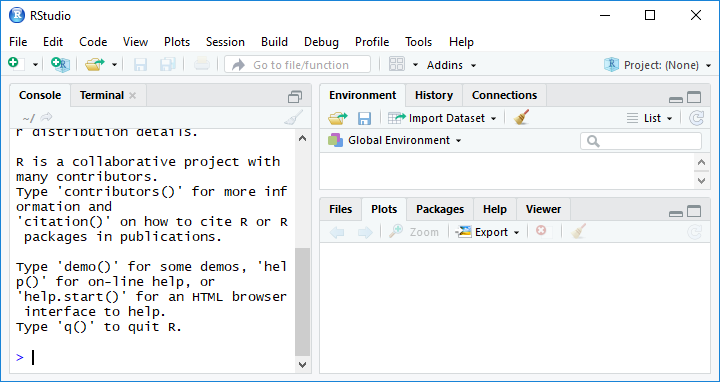
\includegraphics{myFigures/screencap_RStudio_01.png}
\caption{\label{fig:screenCapRStudio01}Captura de pantalla de RStudio en
Windows: pantalla por defecto.\label{fig:screenCapRStudio01}}
\end{figure}

Luego podemos comenzar a escribir nuestro script con los comentarios que
describan lo que vamos a encontrar allí, y agregar un cálculo simple.
Una vez que hayamos copiado el siguiente código, podemos guardar nuestro
script con el comando \texttt{CTRL\ +\ S} o yendo a \emph{Archivo} (o
\emph{File}, luego \emph{Guardar} (o \emph{Save}).

\begin{Shaded}
\begin{Highlighting}[]
\CommentTok{# ------------------------------------------------------------}
\CommentTok{# Un script para seleccionar su entorno de desarrollo}
\CommentTok{# fecha de creación : 27/06/2018}
\CommentTok{# autor : François Rebaudo}
\CommentTok{# ------------------------------------------------------------}

\CommentTok{# [1] cálculos simples}
\CommentTok{# ------------------------------------------------------------}
\NormalTok{nbrRep <-}\StringTok{ }\DecValTok{5}
\NormalTok{pi }\OperatorTok{*}\StringTok{ }\NormalTok{nbrRep}\OperatorTok{^}\DecValTok{2}
\end{Highlighting}
\end{Shaded}

\begin{verbatim}
## [1] 78.53982
\end{verbatim}

Para ejecutar nuestro script, simplemente seleccionamos las líneas que
deseamos ejecutar y usamos la combinación de teclas
\texttt{CTRL\ +\ ENTER}. El resultado aparece en la consola (Figura
\ref{fig:screenCapRStudio02}).

\begin{figure}
\centering
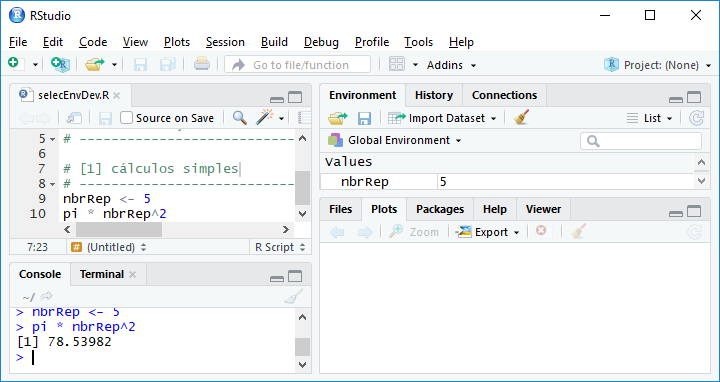
\includegraphics{myFigures/screencap_RStudio_02.png}
\caption{\label{fig:screenCapRStudio02}Captura de pantalla de RStudio en
Windows: ejecutar nuestro script con CTRL +
ENTER.\label{fig:screenCapRStudio02}}
\end{figure}

Podemos ver que, de forma predeterminada, en la parte del script, los
comentarios aparecen en verde, los números en azul y el resto del código
en negro. En la parte de la consola, lo que se ejecutó aparece en azul y
los resultados de la ejecución en negro. También podemos observar que en
la parte del código cada línea tiene un número correspondiente al número
de línea a la izquierda sobre un fondo gris. Este es el resaltado de
preferencias de sintaxis predeterminado con RStudio. Estas preferencias
de sintaxis pueden modificarse yendo al menú \emph{Herramientas} (o
\emph{Tools}), \emph{Opciones globales \ldots{}} (o \emph{Global
Options\ldots{}}), \emph{Aspecto} (o \emph{Appearance}), y luego
seleccionando otro tema del \emph{Editor de tema:} (o \emph{Editor
theme:}). Elegiremos el tema \emph{Cobalt}, luego \emph{OK} (Figura
\ref{fig:screenCapRStudio03}).

\begin{figure}
\centering
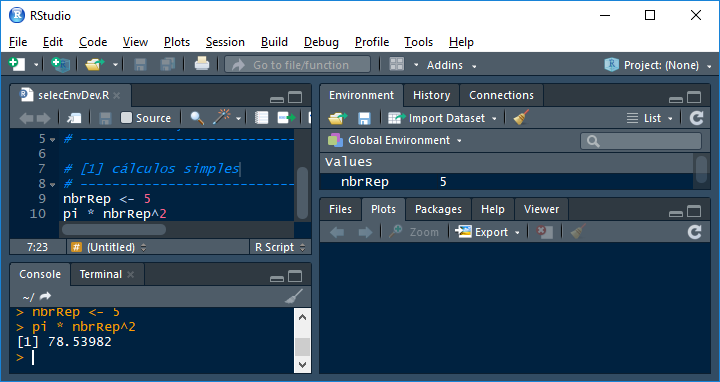
\includegraphics{myFigures/screencap_RStudio_03.png}
\caption{\label{fig:screenCapRStudio03}Captura de pantalla de RStudio en
Windows: cambiar preferencias de
sintaxis.\label{fig:screenCapRStudio03}}
\end{figure}

Sabemos cómo crear un nuevo script, guardarlo, ejecutar su contenido y
cambiar la apariencia de RStudio. Veremos los muchos otros beneficios de
RStudio a lo largo de este libro, ya que es el entorno de desarrollo que
se utilizará. Sin embargo, seremos especialmente cuidadosos de que todos
los scripts desarrollados a lo largo de este libro se ejecuten de la
misma manera, independientemente del entorno de desarrollo utilizado.

\section{Notepad++ avec Npp2R}\label{notepad-avec-npp2r}

\begin{figure}
\centering

\includegraphics{myLogos/Notepadpp.png}
\caption{\label{fig:logoNotepad}Logo Notepad++\label{fig:logoNotepad}}
\end{figure}

\subsection{Instalar Notepad++ (solamente para
Windows)}\label{instalar-notepad-solamente-para-windows}

El programa para instalar Notepad ++ se puede encontrar en la pestaña
\emph{Downloads} (\url{https://notepad-plus-plus.org/download/}).
Podemos elegir entre la versión de 32-bit y la de 64-bit (64-bit si no
sabe qué versión elegir). Notepad++ es suficiente para escribir un
script, pero es aún más poderoso con \emph{Notepad++ to R}
(\emph{Npp2R}) que permite ejecutar automáticamente nuestros scripts en
una consola localmente en nuestra computadora o remotamente en un
servidor.

\subsection{Instalar Npp2R}\label{instalar-npp2r}

El programa para instalar Npp2R está alojado en el sitio de Sourceforge
(\url{https://sourceforge.net/projects/npptor/}). Npp2R debe instalarse
después de Notepad++.

\subsection{Un script con Notepad++}\label{un-script-con-notepad}

Al abrir por primera vez, Notepad++ muestra un archivo vacío \emph{new
1} (Figura \ref{fig:screenCapNpp01}).

\begin{figure}
\centering
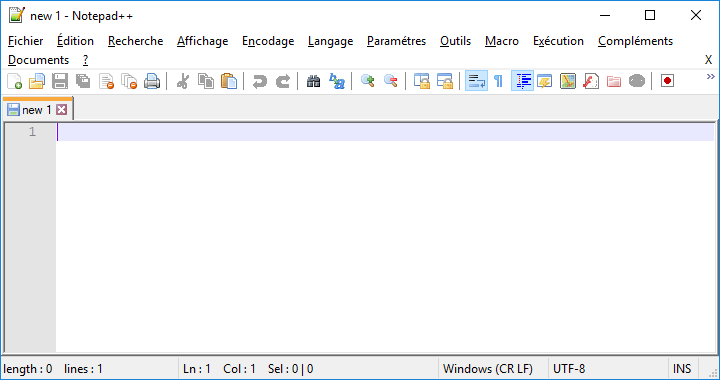
\includegraphics{myFigures/screencap_Npp_01.png}
\caption{\label{fig:screenCapNpp01}Captura de pantalla de Notepad++ en
Windows: pantalla por defecto.\label{fig:screenCapNpp01}}
\end{figure}

Como ya hemos creado un script para probarlo con RStudio, lo abriremos
de nuevo con Notepad++. En \emph{Archivo}, seleccionamos \emph{Abrir
\ldots{}} luego elijemos el script \emph{selecEnvDev.R} creado
previamente. Una vez que el script está abierto, vamos a \emph{Idioma},
luego \emph{R}, y de nuevo \emph{R}. Aparece el resaltado de sintaxis
(Figura \ref{fig:screenCapNpp02}).

\begin{figure}
\centering
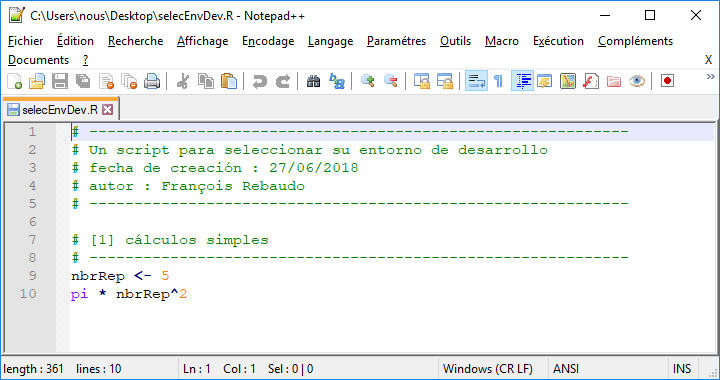
\includegraphics{myFigures/screencap_Npp_02.png}
\caption{\label{fig:screenCapNpp02}Captura de pantalla de Notepad++ en
Windows: ejecutar nuestro script con F8.\label{fig:screenCapNpp02}}
\end{figure}

La ejecución del script solo se puede realizar si se está ejecutando
Npp2R. Para hacerlo, es necesario ejecutar el programa Npp2R desde el
prompt de Windows. Un icono debe aparecer en la parte inferior de su
pantalla demostrando que Npp2R esta prendido. La ejecución automática
del código de Notepad++ se realiza seleccionando el código para ejecutar
y luego usando el comando \texttt{F8}. Si el comando no funciona, puede
ser necesario reiniciar la computadora. Si el comando funciona, se
abrirá una nueva ventana con una consola que ejecuta las líneas deseadas
(Figura \ref{fig:screenCapNpp03}.

\begin{figure}
\centering
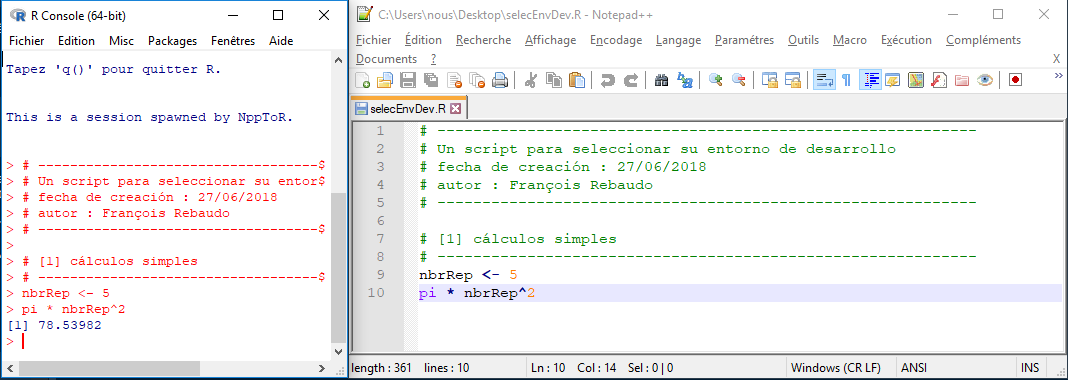
\includegraphics{myFigures/screencap_Npp_03.png}
\caption{\label{fig:screenCapNpp03}Captura de pantalla de Notepad++ en
Windows: la consola con F8.\label{fig:screenCapNpp03}}
\end{figure}

Al igual que con RStudio, el resaltado de sintaxis se puede cambiar
desde el menú \emph{Configuración}, y se puede seleccionar un nuevo tema
(por ejemplo, \emph{Solarized} en la Figura \ref{fig:screenCapNpp04})

\begin{figure}
\centering
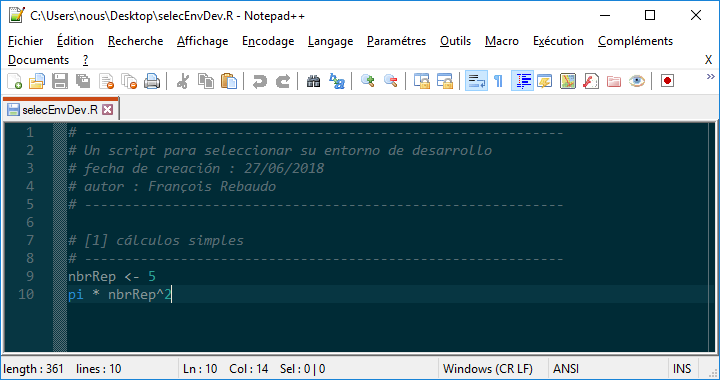
\includegraphics{myFigures/screencap_Npp_04.png}
\caption{\label{fig:screenCapNpp04}Captura de pantalla de Notepad++ en
Windows con el tema Solarized.\label{fig:screenCapNpp04}}
\end{figure}

Comparado con otros editores de texto, Notepad++ tiene la ventaja de ser
muy liviano, rapido y ofrece una amplia gama de opciones para
personalizar la escritura de códigos.

\section{Geany (para Linux, Mac OSX y
Windows)}\label{geany-para-linux-mac-osx-y-windows}

\begin{figure}
\centering

\includegraphics{myLogos/Geany.png}
\caption{\label{fig:logoGeany}Logo Geany\label{fig:logoGeany}}
\end{figure}

\subsection{Instalar Geany}\label{instalar-geany}

El programa para instalar Geany se puede encontrar en la pestaña
\emph{Downloads} en el menú de la izquierda \emph{Releases} de la página
web (\url{https://www.geany.org/}). Luego solo descargamos el ejecutable
para Windows o el dmg para Mac OSX. Los usuarios de Linux preferirán un
\texttt{sudo\ apt-get\ install\ geany}.

\subsection{Un script con Geany}\label{un-script-con-geany}

Al abrir por primera vez, como para RStudio y Notepad++, se crea un
archivo vacío (Figura \ref{fig:screenCapGeany01}).

\begin{figure}
\centering
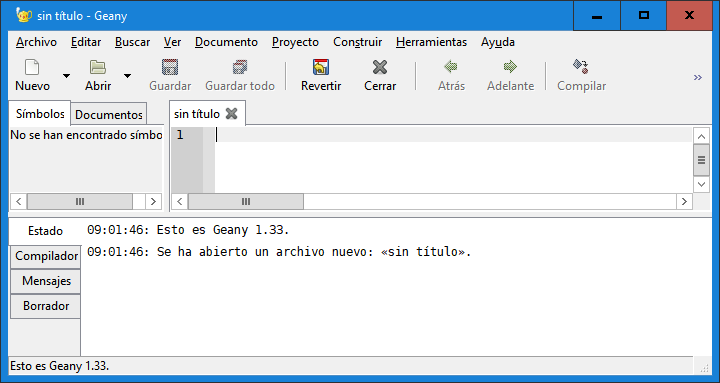
\includegraphics{myFigures/screencap_Geany_01.png}
\caption{\label{fig:screenCapGeany01}Captura de pantalla de Geany en
Windows: pantalla por defecto.\label{fig:screenCapGeany01}}
\end{figure}

Podemos abrir nuestro script con \emph{Archivo}, \emph{Abrir} (Figura
\ref{fig:screenCapGeany02}).

\begin{figure}
\centering
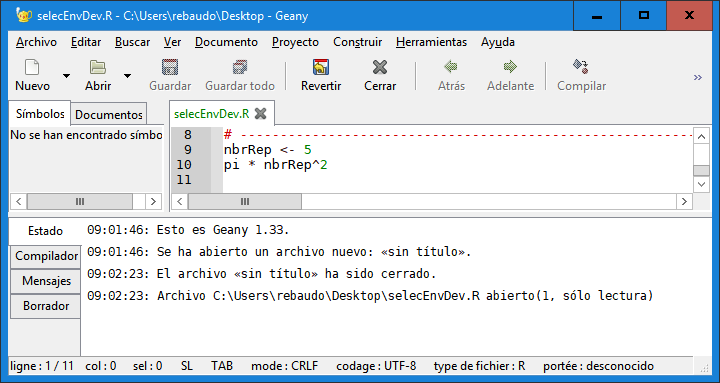
\includegraphics{myFigures/screencap_Geany_02.png}
\caption{\label{fig:screenCapGeany02}Captura de pantalla de Geany en
Windows: abrir un script.\label{fig:screenCapGeany02}}
\end{figure}

Para ejecutar nuestro script, la versión de Geany para Windows no tiene
un terminal incorporado, lo que hace que su uso sea limitado bajo este
sistema operativo. La ejecución de un script se puede hacer abriendo R
en una ventana separada y copiando y pegando las líneas que se
ejecutarán. En Linux y Mac OSX, abramos R en el terminal en la parte
inferior de la ventana de Geany con el comando \texttt{R}. Podemos
configurar Geany para una combinación de teclas para ejecutar el código
seleccionado (por ejemplo \texttt{CTRL\ +\ R}). A esto hay que permitir
el envío de selección al terminal
(\texttt{send\_selection\_unsafe\ =\ true}) in
\texttt{archivo\ geany.conf} y elegir el comando para enviar al terminal
(en \emph{Editar}, \emph{Preferencias}, \emph{Combinaciones}). Para
cambiar el tema de Geany, hay una colección de temas disponibles en
GitHub (\url{https://github.com/geany/geany-themes/}). El tema se puede
cambiar a través del menú \emph{Ver}, \emph{cambiar Esquema del color
\ldots{}} (un ejemplo con el tema \emph{Solarized} Figura @ref(Fig:
screenCapGeany03)).

\begin{figure}
\centering
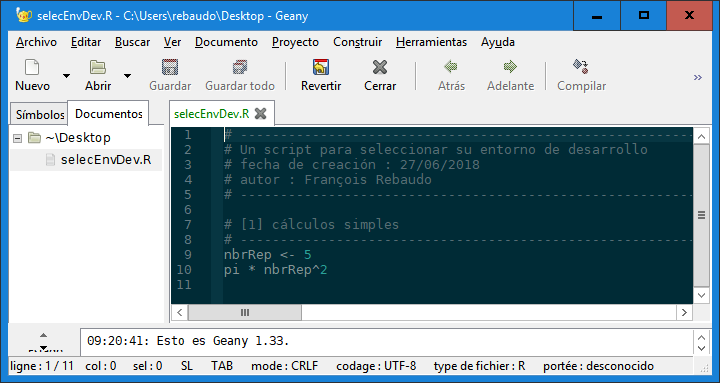
\includegraphics{myFigures/screencap_Geany_03.png}
\caption{\label{fig:screenCapGeany03}Captura de pantalla de Geany en
Windows: cambiar esquema de color.\label{fig:screenCapGeany03}}
\end{figure}

\section{Otras soluciones}\label{otras-soluciones}

Hay muchas otras soluciones, algunas especializadas para R como
\textbf{Tinn-R} (\url{https://sourceforge.net/projects/tinn-r/}), y
otras más generales para programación como \textbf{Atom}
(\url{https://atom.io/}), \textbf{Sublime Text}
(\url{https://www.sublimetext.com/}), \textbf{Vim}
(\url{https://www.vim.org/}), \textbf{Gedit}
(\url{https://wiki.gnome.org/Apps/Gedit}), \textbf{GNU Emacs}
(\url{https://www.gnu.org/software/emacs/}), o \textbf{Brackets}
(\url{http://brackets.io/}) y \textbf{Eclipse}
(\url{http://www.eclipse.org/}).

\section{Conclusion}\label{conclusion-1}

Felicitations, nous sommes arrivés au bout de ce chapitre sur
environnements de développement pour utiliser R. Nous savons désormais :

\begin{itemize}
\tightlist
\item
  Installer RStudio, Geany ou Notepad++
\item
  Reconnaître et choisir notre environnement préféré
\end{itemize}

A partir d'ici nous allons pouvoir nous concentrer sur le language de
programmation R dans un environnement facilitant le travail de lecture
et d'écriture du code. C'est un grand pas en avant pour maîtriser R.

\chapter{Tipos de datos}\label{dataType1}

Vimos anteriormente cómo crear un objeto. Un objeto es como una caja en
la que almacenaremos \emph{información}. Hasta ahora solo hemos
almacenado números, pero en este capítulo veremos que es posible
almacenar otra información y nos detendremos en los tipos más comunes.
En este capítulo utilizaremos \textbf{funciones} sobre las cuales
volveremos más adelante.

\section{\texorpdfstring{El tipo
\texttt{numeric}}{El tipo numeric}}\label{el-tipo-numeric}

El tipo \texttt{numeric} es lo que hemos hecho hasta ahora, almacenando
números. Hay dos tipos principales de números con R: enteros
(\emph{integer}) y números decimales (\emph{double}). Por defecto, R
considera todos los números como números decimales y asigna el tipo
\texttt{double}. Para verificar el tipo de datos utilizaremos la
\emph{función} \texttt{typeof()} que toma como \emph{argumento} un
objeto (o directamente la información que queremos probar). También
podemos usar la función \texttt{is.double()} que devolverá \texttt{TRUE}
si el número está en formato \texttt{double} y \texttt{FALSE} en caso
contrario. La función genérica \texttt{is.numeric()} devolverá
\texttt{TRUE} si el objeto está en formato\texttt{numérico} y
\texttt{FALSE} en caso contrario.

\begin{Shaded}
\begin{Highlighting}[]
\NormalTok{nbrRep <-}\StringTok{ }\DecValTok{5}
\KeywordTok{typeof}\NormalTok{(nbrRep)}
\end{Highlighting}
\end{Shaded}

\begin{verbatim}
## [1] "double"
\end{verbatim}

\begin{Shaded}
\begin{Highlighting}[]
\KeywordTok{typeof}\NormalTok{(}\FloatTok{5.32}\NormalTok{)}
\end{Highlighting}
\end{Shaded}

\begin{verbatim}
## [1] "double"
\end{verbatim}

\begin{Shaded}
\begin{Highlighting}[]
\KeywordTok{is.numeric}\NormalTok{(}\DecValTok{5}\NormalTok{)}
\end{Highlighting}
\end{Shaded}

\begin{verbatim}
## [1] TRUE
\end{verbatim}

\begin{Shaded}
\begin{Highlighting}[]
\KeywordTok{is.double}\NormalTok{(}\DecValTok{5}\NormalTok{)}
\end{Highlighting}
\end{Shaded}

\begin{verbatim}
## [1] TRUE
\end{verbatim}

Si queremos decirle a R que vamos a trabajar con un entero, entonces
necesitamos convertir nuestro número decimal en un entero con la función
\texttt{as.integer()}. También podemos usar la función
\texttt{is.integer()} que devolverá \texttt{TRUE} si el número está en
formato \texttt{integer} y \texttt{FALSE} en caso contrario.

\begin{Shaded}
\begin{Highlighting}[]
\NormalTok{nbrRep <-}\StringTok{ }\KeywordTok{as.integer}\NormalTok{(}\DecValTok{5}\NormalTok{)}
\KeywordTok{typeof}\NormalTok{(nbrRep)}
\end{Highlighting}
\end{Shaded}

\begin{verbatim}
## [1] "integer"
\end{verbatim}

\begin{Shaded}
\begin{Highlighting}[]
\KeywordTok{typeof}\NormalTok{(}\FloatTok{5.32}\NormalTok{)}
\end{Highlighting}
\end{Shaded}

\begin{verbatim}
## [1] "double"
\end{verbatim}

\begin{Shaded}
\begin{Highlighting}[]
\KeywordTok{typeof}\NormalTok{(}\KeywordTok{as.integer}\NormalTok{(}\FloatTok{5.32}\NormalTok{))}
\end{Highlighting}
\end{Shaded}

\begin{verbatim}
## [1] "integer"
\end{verbatim}

\begin{Shaded}
\begin{Highlighting}[]
\KeywordTok{as.integer}\NormalTok{(}\FloatTok{5.32}\NormalTok{)}
\end{Highlighting}
\end{Shaded}

\begin{verbatim}
## [1] 5
\end{verbatim}

\begin{Shaded}
\begin{Highlighting}[]
\KeywordTok{as.integer}\NormalTok{(}\FloatTok{5.99}\NormalTok{)}
\end{Highlighting}
\end{Shaded}

\begin{verbatim}
## [1] 5
\end{verbatim}

\begin{Shaded}
\begin{Highlighting}[]
\KeywordTok{is.numeric}\NormalTok{(nbrRep)}
\end{Highlighting}
\end{Shaded}

\begin{verbatim}
## [1] TRUE
\end{verbatim}

Vemos aquí que convertir un número como \texttt{5.99} a \texttt{entero}
solo devolverá la parte entera, \texttt{5}.

\begin{Shaded}
\begin{Highlighting}[]
\KeywordTok{is.integer}\NormalTok{(}\DecValTok{5}\NormalTok{)}
\end{Highlighting}
\end{Shaded}

\begin{verbatim}
## [1] FALSE
\end{verbatim}

\begin{Shaded}
\begin{Highlighting}[]
\KeywordTok{is.numeric}\NormalTok{(}\DecValTok{5}\NormalTok{)}
\end{Highlighting}
\end{Shaded}

\begin{verbatim}
## [1] TRUE
\end{verbatim}

\begin{Shaded}
\begin{Highlighting}[]
\KeywordTok{is.integer}\NormalTok{(}\KeywordTok{as.integer}\NormalTok{(}\DecValTok{5}\NormalTok{))}
\end{Highlighting}
\end{Shaded}

\begin{verbatim}
## [1] TRUE
\end{verbatim}

\begin{Shaded}
\begin{Highlighting}[]
\KeywordTok{is.numeric}\NormalTok{(}\KeywordTok{as.integer}\NormalTok{(}\DecValTok{5}\NormalTok{))}
\end{Highlighting}
\end{Shaded}

\begin{verbatim}
## [1] TRUE
\end{verbatim}

La suma de un entero y un número de punto flotante devuelve un número de
coma flotante.

\begin{Shaded}
\begin{Highlighting}[]
\NormalTok{sumIntDou <-}\StringTok{ }\KeywordTok{as.integer}\NormalTok{(}\DecValTok{5}\NormalTok{) }\OperatorTok{+}\StringTok{ }\FloatTok{5.2}
\KeywordTok{typeof}\NormalTok{(sumIntDou)}
\end{Highlighting}
\end{Shaded}

\begin{verbatim}
## [1] "double"
\end{verbatim}

\begin{Shaded}
\begin{Highlighting}[]
\NormalTok{sumIntInt <-}\StringTok{ }\KeywordTok{as.integer}\NormalTok{(}\DecValTok{5}\NormalTok{) }\OperatorTok{+}\StringTok{ }\KeywordTok{as.integer}\NormalTok{(}\DecValTok{5}\NormalTok{)}
\KeywordTok{typeof}\NormalTok{(sumIntInt)}
\end{Highlighting}
\end{Shaded}

\begin{verbatim}
## [1] "integer"
\end{verbatim}

Para resumir, el tipo \texttt{numeric} contiene dos subtipos, los tipos
\texttt{integer} para enteros y el tipo \texttt{double} para los números
decimales. Por defecto, R asigna el tipo \texttt{double} a los números.

\section{\texorpdfstring{El tipo
\texttt{character}}{El tipo character}}\label{el-tipo-character}

El tipo \texttt{character} es texto. De hecho, R permite trabajar con
texto. para especificar a R que la información contenida en un objeto
está en formato de texto (o generalmente para todos los textos), usamos
las comillas dobles (\texttt{"}) o las comillas simples
(\texttt{\textquotesingle{}}).

\begin{Shaded}
\begin{Highlighting}[]
\NormalTok{myText <-}\StringTok{ "azerty"}
\NormalTok{myText2 <-}\StringTok{ 'azerty'}
\NormalTok{myText3 <-}\StringTok{ 'azerty uiop qsdfg hjklm'}
\KeywordTok{typeof}\NormalTok{(myText3)}
\end{Highlighting}
\end{Shaded}

\begin{verbatim}
## [1] "character"
\end{verbatim}

Las comillas dobles o simples son útiles si desea poner comillas en
nuestro texto. También podemos \emph{escapar} un carácter especial como
comillas gracias al signo de barra invertida \texttt{\textbackslash{}}.

\begin{Shaded}
\begin{Highlighting}[]
\NormalTok{myText <-}\StringTok{ "a 'ze' 'rt' y"}
\NormalTok{myText2 <-}\StringTok{ 'a "zert" y'}
\NormalTok{myText3 <-}\StringTok{ 'azerty uiop qsdfg hjklm'}
\NormalTok{myText4 <-}\StringTok{ "qwerty }\CharTok{\textbackslash{}"}\StringTok{ azerty "}
\NormalTok{myText5 <-}\StringTok{ "qwerty }\CharTok{\textbackslash{}\textbackslash{}}\StringTok{ azerty "}
\end{Highlighting}
\end{Shaded}

De forma predeterminada, cuando creamos un objeto, su contenido no es
devuelto por la consola. En Internet o en muchos libros podemos
encontrar el nombre del objeto en una línea para devolver sus
contenidos:

\begin{Shaded}
\begin{Highlighting}[]
\NormalTok{myText <-}\StringTok{ "a 'ze' 'rt' y"}
\NormalTok{myText}
\end{Highlighting}
\end{Shaded}

\begin{verbatim}
## [1] "a 'ze' 'rt' y"
\end{verbatim}

En este libro, no lo usaremos de esta manera y preferiremos el uso de la
función \texttt{print()}, que permite mostrar en la consola el contenido
de un objeto. El resultado es el mismo, pero el código es más fácil de
leer y más explícito sobre lo que hace.

\begin{Shaded}
\begin{Highlighting}[]
\NormalTok{myText <-}\StringTok{ "a 'ze' 'rt' y"}
\KeywordTok{print}\NormalTok{(myText)}
\end{Highlighting}
\end{Shaded}

\begin{verbatim}
## [1] "a 'ze' 'rt' y"
\end{verbatim}

\begin{Shaded}
\begin{Highlighting}[]
\NormalTok{nbrRep <-}\StringTok{ }\DecValTok{5}
\KeywordTok{print}\NormalTok{(nbrRep)}
\end{Highlighting}
\end{Shaded}

\begin{verbatim}
## [1] 5
\end{verbatim}

También podemos poner números en formato de texto, pero no debemos
olvidar poner comillas para especificar el tipo \texttt{character} o
usar la función\texttt{as.character()}. Una operación entre un texto y
un número devuelve un error. Por ejemplo, si agregamos \texttt{10} a
\texttt{5}, R nos dice que un \textbf{argumento} de la \textbf{función}
\texttt{+} no es un tipo \texttt{numeric} y que, por lo tanto, la
operación no es posible. Tampoco podemos agregar texto a texto, pero
veremos más adelante cómo \emph{concatenar} dos cadenas de texto.

\begin{Shaded}
\begin{Highlighting}[]
\NormalTok{myText <-}\StringTok{ "qwerty"}
\KeywordTok{typeof}\NormalTok{(myText)}
\end{Highlighting}
\end{Shaded}

\begin{verbatim}
## [1] "character"
\end{verbatim}

\begin{Shaded}
\begin{Highlighting}[]
\NormalTok{myText2 <-}\StringTok{ }\DecValTok{5}
\KeywordTok{typeof}\NormalTok{(myText2)}
\end{Highlighting}
\end{Shaded}

\begin{verbatim}
## [1] "double"
\end{verbatim}

\begin{Shaded}
\begin{Highlighting}[]
\NormalTok{myText3 <-}\StringTok{ "5"}
\KeywordTok{typeof}\NormalTok{(myText3)}
\end{Highlighting}
\end{Shaded}

\begin{verbatim}
## [1] "character"
\end{verbatim}

\begin{Shaded}
\begin{Highlighting}[]
\NormalTok{myText2 }\OperatorTok{+}\StringTok{ }\DecValTok{10}
\end{Highlighting}
\end{Shaded}

\begin{verbatim}
## [1] 15
\end{verbatim}

\begin{Shaded}
\begin{Highlighting}[]
\KeywordTok{as.character}\NormalTok{(}\DecValTok{5}\NormalTok{)}
\end{Highlighting}
\end{Shaded}

\begin{verbatim}
## [1] "5"
\end{verbatim}

\begin{Shaded}
\begin{Highlighting}[]
\CommentTok{# myText3 + 10 # Error in myText3 + 10 : non-numeric argument to binary operator}
\CommentTok{# "a" + "b" # Error in "a" + "b" : non-numeric argument to binary operator}
\end{Highlighting}
\end{Shaded}

Para resumir, el tipo \texttt{character} permite el ingreso de texto,
podemos reconocerlo con comillas simples o dobles.

\section{\texorpdfstring{El tipo
\texttt{factor}}{El tipo factor}}\label{el-tipo-factor}

El tipo \texttt{factor} corresponde a los factores. Los factores son una
elección dentro de una lista finita de posibilidades. Por ejemplo, los
países son factores porque existe una lista finita de países en el mundo
en un momento dado. Un factor puede definirse con la función
\texttt{factor()} o transformarse utilizando la función
\texttt{as.factor()}. Al igual que con otros tipos de datos, podemos
usar la función \texttt{is.factor()} para verificar el tipo de datos.
Para obtener una lista de todas las posibilidades, existe la función
\texttt{levels()} (esta función tendrá más sentido cuando nos acerquemos
a los tipos de contenedores de información).

\begin{Shaded}
\begin{Highlighting}[]
\NormalTok{factor01 <-}\StringTok{ }\KeywordTok{factor}\NormalTok{(}\StringTok{"aaa"}\NormalTok{)}
\KeywordTok{print}\NormalTok{(factor01)}
\end{Highlighting}
\end{Shaded}

\begin{verbatim}
## [1] aaa
## Levels: aaa
\end{verbatim}

\begin{Shaded}
\begin{Highlighting}[]
\KeywordTok{typeof}\NormalTok{(factor01)}
\end{Highlighting}
\end{Shaded}

\begin{verbatim}
## [1] "integer"
\end{verbatim}

\begin{Shaded}
\begin{Highlighting}[]
\KeywordTok{is.factor}\NormalTok{(factor01)}
\end{Highlighting}
\end{Shaded}

\begin{verbatim}
## [1] TRUE
\end{verbatim}

\begin{Shaded}
\begin{Highlighting}[]
\KeywordTok{levels}\NormalTok{(factor01)}
\end{Highlighting}
\end{Shaded}

\begin{verbatim}
## [1] "aaa"
\end{verbatim}

Un factor se puede transformar en texto con la función
\texttt{as.character()} pero también en número con
\texttt{as.numeric()}. Al cambiar al tipo \texttt{numeric}, cada factor
toma el valor de su posición en la lista de posibilidades. En nuestro
caso, solo hay una posibilidad, por lo que la función
\texttt{as.numeric()} devolverá \texttt{1}:

\begin{Shaded}
\begin{Highlighting}[]
\NormalTok{factor01 <-}\StringTok{ }\KeywordTok{factor}\NormalTok{(}\StringTok{"aaa"}\NormalTok{)}
\KeywordTok{as.character}\NormalTok{(factor01)}
\end{Highlighting}
\end{Shaded}

\begin{verbatim}
## [1] "aaa"
\end{verbatim}

\begin{Shaded}
\begin{Highlighting}[]
\KeywordTok{as.numeric}\NormalTok{(factor01)}
\end{Highlighting}
\end{Shaded}

\begin{verbatim}
## [1] 1
\end{verbatim}

\section{\texorpdfstring{El tipo
\texttt{logical}}{El tipo logical}}\label{el-tipo-logical}

El tipo \texttt{logical} corresponde a los valores \texttt{TRUE} y
\texttt{FALSE} (y \texttt{NA}) que ya hemos visto con los operadores de
comparación.

\begin{Shaded}
\begin{Highlighting}[]
\NormalTok{aLogic <-}\StringTok{ }\OtherTok{TRUE}
\KeywordTok{print}\NormalTok{(aLogic)}
\end{Highlighting}
\end{Shaded}

\begin{verbatim}
## [1] TRUE
\end{verbatim}

\begin{Shaded}
\begin{Highlighting}[]
\KeywordTok{typeof}\NormalTok{(aLogic)}
\end{Highlighting}
\end{Shaded}

\begin{verbatim}
## [1] "logical"
\end{verbatim}

\begin{Shaded}
\begin{Highlighting}[]
\KeywordTok{is.logical}\NormalTok{(aLogic)}
\end{Highlighting}
\end{Shaded}

\begin{verbatim}
## [1] TRUE
\end{verbatim}

\begin{Shaded}
\begin{Highlighting}[]
\NormalTok{aLogic }\OperatorTok{+}\StringTok{ }\DecValTok{1}
\end{Highlighting}
\end{Shaded}

\begin{verbatim}
## [1] 2
\end{verbatim}

\begin{Shaded}
\begin{Highlighting}[]
\KeywordTok{as.numeric}\NormalTok{(aLogic)}
\end{Highlighting}
\end{Shaded}

\begin{verbatim}
## [1] 1
\end{verbatim}

\begin{Shaded}
\begin{Highlighting}[]
\KeywordTok{as.character}\NormalTok{(aLogic)}
\end{Highlighting}
\end{Shaded}

\begin{verbatim}
## [1] "TRUE"
\end{verbatim}

\section{\texorpdfstring{Acerca de
\texttt{NA}}{Acerca de NA}}\label{acerca-de-na}

El valor \texttt{NA} se puede usar para especificar que no hay datos o
datos faltantes. Por defecto, \texttt{NA} es \texttt{logical}, pero se
puede usar para texto o números.

\begin{Shaded}
\begin{Highlighting}[]
\KeywordTok{print}\NormalTok{(}\OtherTok{NA}\NormalTok{)}
\end{Highlighting}
\end{Shaded}

\begin{verbatim}
## [1] NA
\end{verbatim}

\begin{Shaded}
\begin{Highlighting}[]
\KeywordTok{typeof}\NormalTok{(}\OtherTok{NA}\NormalTok{)}
\end{Highlighting}
\end{Shaded}

\begin{verbatim}
## [1] "logical"
\end{verbatim}

\begin{Shaded}
\begin{Highlighting}[]
\KeywordTok{typeof}\NormalTok{(}\KeywordTok{as.integer}\NormalTok{(}\OtherTok{NA}\NormalTok{))}
\end{Highlighting}
\end{Shaded}

\begin{verbatim}
## [1] "integer"
\end{verbatim}

\begin{Shaded}
\begin{Highlighting}[]
\KeywordTok{typeof}\NormalTok{(}\KeywordTok{as.character}\NormalTok{(}\OtherTok{NA}\NormalTok{))}
\end{Highlighting}
\end{Shaded}

\begin{verbatim}
## [1] "character"
\end{verbatim}

\begin{Shaded}
\begin{Highlighting}[]
\OtherTok{NA} \OperatorTok{==}\StringTok{ }\OtherTok{TRUE}
\end{Highlighting}
\end{Shaded}

\begin{verbatim}
## [1] NA
\end{verbatim}

\begin{Shaded}
\begin{Highlighting}[]
\OtherTok{NA} \OperatorTok{==}\StringTok{ }\OtherTok{FALSE}
\end{Highlighting}
\end{Shaded}

\begin{verbatim}
## [1] NA
\end{verbatim}

\begin{Shaded}
\begin{Highlighting}[]
\OtherTok{NA} \OperatorTok{>}\StringTok{ }\DecValTok{1}
\end{Highlighting}
\end{Shaded}

\begin{verbatim}
## [1] NA
\end{verbatim}

\begin{Shaded}
\begin{Highlighting}[]
\OtherTok{NA} \OperatorTok{+}\StringTok{ }\DecValTok{1}
\end{Highlighting}
\end{Shaded}

\begin{verbatim}
## [1] NA
\end{verbatim}

\section{Conclusión}\label{conclusion-1}

Felicitaciones, hemos llegado al final de este capítulo sobre los tipos
de datos. Ahora sabemos:

\begin{itemize}
\tightlist
\item
  Reconocer y hacer objetos en los principales tipos de datos
\item
  Transformar tipos de datos de un tipo a otro
\end{itemize}

Este capítulo bastante tedioso es la base para el próximo capítulo sobre
contenedores de datos.

\chapter{Contenedores de datos}\label{dataType2}

\section{\texorpdfstring{El contenedor
\texttt{vector}}{El contenedor vector}}\label{el-contenedor-vector}

XXX

\section{\texorpdfstring{El contenedor
\texttt{list}}{El contenedor list}}\label{el-contenedor-list}

XXX

\section{\texorpdfstring{El contenedor
\texttt{data.frame}}{El contenedor data.frame}}\label{el-contenedor-data.frame}

XXX

\section{\texorpdfstring{El contenedor
\texttt{matrix}}{El contenedor matrix}}\label{el-contenedor-matrix}

XXX

\section{\texorpdfstring{El contenedor
\texttt{array}}{El contenedor array}}\label{el-contenedor-array}

XXX

\chapter{Las funciones}\label{fonctions}

\section{¿Qué es una función?}\label{que-es-una-funcion}

XXX

\section{Las funciones más comunes}\label{las-funciones-mas-comunes}

\subsection{Ver los datos}\label{ver-los-datos}

str head tail class

\subsection{funciones matemáticas}\label{funciones-matematicas}

exp sqrt

\subsection{Estadísticas descriptivas}\label{estadisticas-descriptivas}

mean sd max min quartile summary meadian

\section{Otras funciones útiles}\label{otras-funciones-utiles}

XXX

\section{Escribe una función}\label{escribe-una-funcion}

XXX

\chapter{Importar y exportar datos}\label{import}

\section{Leer datos de un archivo}\label{leer-datos-de-un-archivo}

XXX

\section{Guardar datos para R}\label{guardar-datos-para-r}

save load

\section{Exportar datos}\label{exportar-datos}

write XXX

\chapter{Los bucles}\label{loops}

\section{¿Por qué hacer bucles?}\label{por-que-hacer-bucles}

XXX algorítmico \ldots{}

\section{\texorpdfstring{El bucle
\texttt{if}}{El bucle if}}\label{el-bucle-if}

XXX

\section{\texorpdfstring{El bucle
\texttt{switch}}{El bucle switch}}\label{el-bucle-switch}

XXX

\section{\texorpdfstring{El bucle
\texttt{for}}{El bucle for}}\label{el-bucle-for}

XXX

\section{\texorpdfstring{El bucle
\texttt{while}}{El bucle while}}\label{el-bucle-while}

XXX

\section{\texorpdfstring{\texttt{repeat}, \texttt{next}, \texttt{break},
\texttt{stop}}{repeat, next, break, stop}}\label{repeat-next-break-stop}

XXX

\section{\texorpdfstring{Los bucles de la familia
\texttt{apply}}{Los bucles de la familia apply}}\label{los-bucles-de-la-familia-apply}

\subsection{\texorpdfstring{\texttt{apply}}{apply}}\label{apply}

XXX

\subsection{\texorpdfstring{\texttt{sapply}}{sapply}}\label{sapply}

XXX

\subsection{\texorpdfstring{\texttt{lapply}}{lapply}}\label{lapply}

XXX

\subsection{\texorpdfstring{\texttt{tapply}}{tapply}}\label{tapply}

XXX

\subsection{\texorpdfstring{\texttt{mapply}}{mapply}}\label{mapply}

XXX

\part{Los gráficos}\label{part-los-graficos}

\chapter{Gráficos simples}\label{graph1}

\section{plot}\label{plot}

\section{hist}\label{hist}

\section{barplot}\label{barplot}

\section{boxplot}\label{boxplot}

\section{image y contour}\label{image-y-contour}

\chapter{Gestión del color}\label{graph2}

\section{colors()}\label{colors}

\section{RGB}\label{rgb}

\section{Paletas}\label{paletas}

\chapter{Gráficos compuestos}\label{graph3}

\section{mfrow}\label{mfrow}

\section{layout}\label{layout}

\chapter{Manipular gráficos}\label{graph4}

\section{Inkscape}\label{inkscape}

\section{The Gimp}\label{the-gimp}

\part{Estadísticas con R}\label{part-estadisticas-con-r}

\chapter{Estadísticas descriptivas}\label{stats1}

\part{Estudio de caso}\label{part-estudio-de-caso}

\chapter{Analizar datos de loggers de temperatura}\label{studyCase1}


\end{document}
